\chapter{The Laws of the Euclidean Geometries}
\paragraph{Acknowledgements}
Thanks to Cadence Weddle, Leona Liu, and Zoya Yan.
\paragraph{Note}
Please note that all angles are in degrees and all symbolic values are within the set $\{x\in\mathbb{R} \mid x\geq0\}$.
\section*{Primitive Notions}
\begin{enumerate}
    \item Point
    \item Line
    \item Plane
\end{enumerate}

\section*{Definition of Basic Objects}
\begin{enumerate}
     \item A segment is the set of all points between two distinct points (called the endpoints)
     \item A ray is a segment together with the set of all points beyond one of the endpoints
     \item Opposite rays are rays which lie on the same line and whose only point of intersection is their common endpoint
     \item Collinear points are points which lie on the same line\end{enumerate}

\section*{Definitions}
\begin{enumerate}
    \item Property of Betweenness: the whole equals the sum of its parts
    \item Given collinear points $C$, $D$, and $E$, if $D$ is a point between $C$ and $E$, then $CD + DE = CE$.
    \item Midpoint: divides segment into 2 equal parts in half
    \item Segment bisector: meets a segment at its midpoint
    \item Angle Addition Postulate: the whole equals the sum of its parts
    \item Angle bisector: divides an angle into 2 equal parts in half
    \item Complementary angle: 2 angles whose sum is 90 degrees
    \item Supplementary angle: 2 angles whose sum is 180 degrees
    \item Adjacent angles: 2 angles that satisfy the following
    \begin{enumerate}
        \item Common vertex
        \item Common side
        \item Don’t share common interior points
    \end{enumerate}
    \item Vertical angles: 2 non-adjacent angles formed by the intersection of 2 lines
    \item The distance between a point and a line (or subset of a line) is the length of the segment perpendicular to the line with the point as an endpoint
\end{enumerate}

\section*{Properties}
\begin{enumerate}
    \item All vertical angles are equal
    \item Substitution: $\forall a,b,c,d\in X:(a=b\wedge a=c\wedge b=d)\Rightarrow (c=d)$
    \item Transitive: $\forall a,b,c\in X:(aRb\wedge bRc)\Rightarrow aRc$ where $R$ is some equality operator.
    \item Reflexive Property
    \item Addition Property of Equality
    \item Subtraction Property of Equality
    \item Division Property of Equality: halves of equals are equal
    \item Multiplication Property of Equality
\end{enumerate}

\section*{Perpendicularity and Right Angles}
\begin{enumerate}
    \item If 2 lines meet to form 2 equal adjacent angles, then the lines are perpendicular
    \item Perpendicular lines meet to form right angles
    \item All right angles are equal
\end{enumerate}

\section*{Complements and Supplements}
\begin{enumerate}
    \item If the exterior sides of 2 adjacent angles are opposite rays, then the angles are supplementary
    \item If the exterior sides of 2 adjacent angles are perpendicular, then the angles are complementary
    \item If 2 angles are complementary to the same angle, then they are equal to each other
    \item If 2 angles are complementary to equal angles, then they are equal to each other
    \item If 2 angles are supplementary to the same angle, then are equal to each other
    \item If 2 angles are supplementary to equal angles, then are equal to each other
\end{enumerate}

\section*{Triangle Congruence}
\begin{enumerate}
    \item SSS (side-side-side)
    \item SAS (side-angle-side)
    \item ASA (angle-side-angle)
    \item AAS (angle-angle-side)
    \item RHL (right-hypotenuse-leg)
    \item CPCTE: Corresponding Parts of Congruent Triangles are Equal
\end{enumerate}

\section*{Triangles}
\begin{enumerate}
    \item Median: a segment drawn from the vertex of a triangle to the midpoint of the opposite side
    \item Altitude: a segment drawn from a vertex of a triangle perpendicular to the opposite side
    \item The sum of the interior angles of a triangle is 180 degrees
\end{enumerate}

\section*{Isosceles Triangles}
\begin{enumerate}
    \item If a triangle has 2 equal sides, then it is isosceles
    \item In a triangle, if 2 sides are equal, then the 2 angles opposite them are equal
    \item In a triangle, if 2 angles are equal then the 2 sides opposite them are equal
    \item An exterior angle of a triangle equals the sum of its remote interior angles
    \item In an isosceles triangle, the median is an altitude
\end{enumerate}
\section*{Inequality}
\begin{enumerate}
    \item A whole is greater than either one of its parts
    \item In a triangle, the greater angle lies opposite the greater side
    \item Transitive property of inequality: $\forall a,b,c\in X:(aRb\wedge bRc)\Rightarrow aRc$ where $R$ is some inequality operator.
    \item An exterior angle of a triangle is greater than either of its remote angles
\end{enumerate}

\section*{Parallel Lines and Transversals}
\begin{enumerate}
    \item Parallel lines: 2 coplanar lines which never intersect
    \item Transversal: a line that intersects 2 other lines in 2 distinct locations
    \item Alternate interior angles: non-adjacent angles in the interior of a transversal on opposite sides
    \item Same-side interior angles: non-adjacent angles in the interior of a transversal on the same side
    \item Corresponding angles definition: one interior and one exterior non-adjacent angle on the same side of the transversal
    \item If alternate interior angles are equal, then the lines are parallel
    \item If corresponding angles are equal, then the lines are parallel
    \item If same side interior angles are supplementary, then the lines are parallel
    \item If 2 lines are perpendicular to the same line, then they are parallel
    \item Parallel Postulate: Through a point not on a given line, there exists one and only one line parallel to the given line
    \item If lines are parallel, then alternate interior angles are equal
    \item If lines are parallel, then corresponding angles are equal
    \item If lines are parallel, then same side interior angles are supplementary
    \item If 2 lines are parallel to the same line, then they are parallel to each other
    \item If 3 or more parallel lines cut off equal segments on a transversal, then they do so on any transversal
\end{enumerate}

\section*{Midline/Midsegment}
\begin{enumerate}
    \item A midline is a segment which connects the midpoints of 2 sides of a triangle
    \item A midline is parallel to the third side
    \item A midline is half the length of the third side
    \item If a line is drawn from the midpoint of a side of a triangle and is parallel to another side, then it intersects the 3rd side of the triangle at its midpoint
\end{enumerate}

\section*{Parallelogram Properties}
\begin{enumerate}
    \item A diagonal is a segment that is formed by connecting 2 non-connecting two nonconsecutive vertical angles
    \item A parallelogram is a quadrilateral where both pairs of opposite sides are parallel
    \item If a quadrilateral is a parallelogram, then opposite sides are equal
    \item If a quadrilateral is a parallelogram, then opposite angles are equal
    \item If a quadrilateral is a parallelogram the diagonals bisect each other
\end{enumerate}

\section*{Parallelogram Converses}
\begin{enumerate}
    \item If both pairs of opposite sides are parallel, then a quadrilateral is a parallelogram
    \item If both pairs of opposite sides are equal, then a quadrilateral is a parallelogram
    \item If both pairs of opposite angles are equal, then a quadrilateral is a parallelogram
    \item If diagonals bisect each other, then a quadrilateral is a parallelogram
    \item If the same pair of opposite sides is both parallel and equal, then a quadrilateral is a parallelogram
\end{enumerate}

\section*{Rectangle Properties}
\begin{enumerate}
    \item \# Inherit from Parallelogram
    \item Rectangle: parallelogram with a right angle
    \item A rectangle has all right angles
    \item A rectangle is equiangular
    \item A rectangle has equal diagonals
    \item Rectangle Converses
    \item If a parallelogram has a right angle, then it is a rectangle
    \item If a quadrilateral is equiangular, then it is a rectangle
    \item If a parallelogram has equal diagonals, then it is a rectangle
\end{enumerate}


\section*{Rhombus Properties}
\begin{enumerate}
    \item \#Inherit from Parallelogram
    \item A rhombus is a parallelogram with 2 equal consecutive sides
    \item A rhombus is equilateral
    \item A rhombus has diagonals that bisect the angles
    \item A rhombus has perpendicular diagonals
    \item Rhombus Converses
    \item A parallelogram with 2 equal consecutive angles is a rhombus
    \item If a quadrilateral is equilateral, then it is a rhombus
    \item If the diagonals of a parallelogram bisect an angle, then it is a rhombus
    \item If the diagonals of a parallelogram are perpendicular, then it is a rhombus
\end{enumerate}

\section*{Squares}
\begin{enumerate}
    \item \#Inherit from Parallelogram
    \item \#Inherit from Rhombus
    \item \#Inherit from Rectangle
    \item Square: parallelogram with 2 equal consecutive sides and a right angle
    \item A square is a rhombus with a right angle
    \item A square is a rectangle with two equal consecutive sides
\end{enumerate}

\section*{Trapezoids}
\begin{enumerate}
    \item A trapezoid is quadrilateral with exactly one pair of opposite sides parallel
    \item An isosceles trapezoid is a trapezoid with non-parallel sides that are equal
    \item An isosceles trapezoid has base angles that are equal
    \item An isosceles triangle has diagonals that are equal
    \item Median of a trapezoid: segment which connects the midpoints of 2 non-parallel sides
    \item A median of a trapezoid is parallel to both bases of the trapezoid
    \item The measure of the median of a trapezoid is equal to the arithmetic mean of the measures of the bases
\end{enumerate}

\section*{Interior and Exterior Angles of Polygons}
\begin{enumerate}
    \item The sum of the interior angles of a simple convex $n$-gon is $180*(n-2)$ degrees
    \item The sum of the exterior angles of a simple convex $n$-gon is always 360 degrees
\end{enumerate}

\section*{Properties of Proportion}
\begin{enumerate}
    \item Cross Multiplication (Means Extremes Rule) $\frac{a}{b}=\frac{c}{d}\Rightarrow ad=bc$
    \item Alternation $\frac{a}{b}=\frac{c}{d}\Rightarrow\frac{a}{c}=\frac{b}{d}$
    \item Inversion $\frac{a}{b}=\frac{c}{d}\Rightarrow\frac{b}{a}=\frac{d}{c}$
    \item Addition Property of Equality $\frac{a}{b}=\frac{c}{d}\Rightarrow\frac{a + b}{b}=\frac{c + d}{d}$
\end{enumerate}

\section*{Similarity}
\begin{enumerate}
    \item Similar polygons have corresponding angles that are equal
    \item Similar polygons have corresponding sides in proportion
    \item AA(A): Angle Angle Similarity
    \item CASTE: Corresponding Angles of Similar Triangles are Equal
    \item CSSTP: Corresponding Sides of Similar Triangles are Proportional
\end{enumerate}

\section*{Right Triangles and Trigonometry}
\begin{enumerate}
    \item In a right triangle, the midpoint of the hypotenuse is equidistant from all of the vertices
\end{enumerate}

\section*{Triangle Proportionality}
\begin{enumerate}
    \item Triangle Proportionality Theorem: If a line parallel to one side of a triangle intersects the other two sides, then it divides them proportionally
    \item Converse of the Triangle Proportionality Theorem: If a line divides two sides of a triangle proportionally, then it is parallel to the third side
    \item The bisector of an angle of a triangle divides the sides opposite the angle in the ratio of the lengths of the other two sides of the triangle
    \item Three (or more) parallel lines cut off proportional segments on any two transversals
\end{enumerate}

\section*{Proportions in a Right Triangle Divided by an Altitude}
\begin{tikzpicture}
    \draw [thin](-5,0) -- (0,5) node[right,pos=0.5]{$b$};
    \draw [thin](0,5) -- (5,0) node[left,pos=0.5]{$k$};
    \draw [thin](-5,0) -- (0,0) node[below,pos=0.5]{$a$};
    \draw [thin](0,0) -- (5,0) node[below,pos=0.5]{$c$};

    \draw [densely dotted](-0.5,0) -- (-0.5,0.5) -- (0.5,0.5) -- (0.5,0);
    \draw [densely dotted](-0.35355339059327373,4.646446609406726) -- (0,4.292893218813452) -- (0.353553390593273735,4.646446609406726);

    \draw [dash dot](-5,0) -- (-5,-1) -- (5,-1) node[below,pos=0.5]{$f$} -- (5,0) ;
    \draw [dash dot](0,0) -- (0,5) node[left,pos=0.5]{$h$};
\end{tikzpicture}

\begin{enumerate}
    \item $\frac{c}{k}=\frac{k}{f}$
    \item $\frac{a}{b}=\frac{b}{f}$
    \item $\frac{a}{h}=\frac{h}{c}$
\end{enumerate}

\section*{Circle Definitions}
\begin{tikzpicture}
    \draw (0,0) circle (5cm);
    \draw [densely dotted](-5,-5)--(-5,5);
\end{tikzpicture}

\begin{enumerate}
    \item Circle: The set of all points in a plane a given distance from a given point (the center of the circle)
    \item Radius: Any segment whose endpoints are the center and a point on the circle
    \item The length of any such segment is called the radius of the circle
    \item Chord: any segment whose endpoints are two points of a circle
    \item Diameter: A chord that contains the center of the circle
    \item The length of any such segment is called the diameter of the circle
    \item Secant: Any line (or ray or segment) that has as a subset a chord of the circle
    \item Tangent: Any line in the plane of the circle that intersects the circle in exactly one point, called the point of tangency
    \item Concentric circles: Circles in the same plane with the same center but different radii
    \item Congruent circles: Circles with congruent radii
    \item Central angle: An angle whose vertex is the center of the circle
    \item Inscribed angle: An angle whose vertex lies on the circle and whose sides have as subsets chords of the circle
    \item Inscribed polygon: A polygon all of whose vertices lie on the same circle
    \item Quadrilateral ABCD is inscribed in circle O → Circle O is circumscribed about quadrilateral ABCD
    \item Circumscribed polygon: A polygon all of whose sides are tangent to the same circle
    \item If R and Q are endpoints of a diameter of a circle, then R, Q, and either half of the circle with endpoints R and Q is a semicircle
    \item If P and Q are not endpoints of a diameter of O, then the arc consisting of P, Q, and all points in the interior of $\sphericalangle POQ$ is a minor arc of O, denoted ab
    \item If P and Q are not endpoints of a diameter of O, then the arc consisting of P, Q, and all the points on the circle in the exterior of $\sphericalangle POQ$ is a major arc
    \item To name a semicircle or major arc, you must use three letters
    \item An angle intercepts an arc if each side of the angle contains an endpoint of the arc
    \item All other points of the arc lie in the interior of the angle
\end{enumerate}

\section*{Properties of Circle Components}
\begin{enumerate}
    \item Radii of the same circle are equal
    \item The measure of a minor arc is equal to the measure of the central angle that intercepts it
    \item The measure of a semicircle is $180\,^{\circ}$
    \item The measure of an entire circle is $360\,^{\circ}$
    \item The measure of a major arc is the difference between  $360\,^{\circ}$ and the measure of the corresponding minor arc
    \item Two arcs of the same circle or congruent circles are congruent if they have the same measure
    \item An angle inscribed in a semicircle is a right angle
    \item The measure of an inscribed angle is half the measure of its intercepted arc
    \item If a quadrilateral is inscribed within a circle, then angles opposite each other are supplementary
    \item If 2 arcs in a circle are equal, then the inscribed angles which intercept them are equal
    \item If 2 angles of the same type intercept the same arc, then the two angles are equal
    \item If 2 inscribed angles formed by 2 arcs are equal, then the 2 arcs are equal
    \item A tangent to a circle is perpendicular to the radius/diameter drawn to the point of tangency
    \item A tangent-chord angle measures half its intercepted arc
    \item Angles Formed by Intersections of Chords, Tangents, and Secants
    \item An angle formed by two chords measures half the sum of its intercepted arcs
    \item An angle formed by two secants measures half the difference of its intercepted arcs
    \item An angle formed by a secant and a tangent measures half the difference of its intercepted arcs
    \item An angle formed by 2 tangents measures half the difference of its intercepted arcs
    \item An angle formed by 2 tangents measures $180\,^{\circ}$ minus the measure of its intercepted minor arc
\end{enumerate}

\section*{Chord Theorems}
\begin{enumerate}
    \item If 2 chords are parallel, then they cut off equal arcs between them
    \item If 2 chords are equal, then the arcs they cut off are equal
    \item If a radius is drawn perpendicular to a chord, then it bisects the chord (and arc it intersects)
    \item If 2 chords are equal, then they are equidistant from the center of the circle
\end{enumerate}

\section*{Segment Length}
\begin{table}[H]
\caption{An Illustration of the Various Segments related to a Circle}
\centering
\begin{tabular}{c c c c}
\hline
$a\cdot d = c \cdot b$ & $a=b$ & $b\cdot(c+b)=d\cdot(a+d)$ & $a\cdot(a+b)=c^{2}$\\
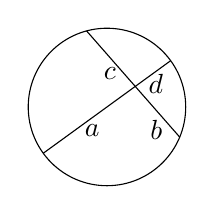
\begin{tikzpicture}
    \draw (0,0) circle (1cm);
    \draw [thin](-0.8090169943749475,-0.5877852522924731)--(0.8090169943749475,0.5877852522924731)node[right,pos=0.25]{$a$} node[right,pos=0.75]{$d$};
    \draw [thin](-0.25881904510252074,0.9659258262890683)--(0.9238795325112867,-0.3826834323650898)node[below,pos=0.25]{$c$} node[below,pos=0.75]{$b$};
\end{tikzpicture}&

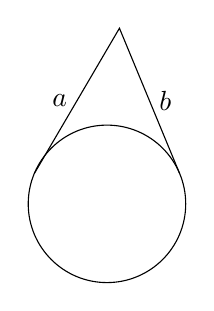
\begin{tikzpicture}
    \draw (0,0) circle (1cm);
    \draw [thin](-0.9238795325112867,0.3826834323650899)--(0.1585126677811072126712632,2.230442497387663283984826)node[left,pos=0.5] {$a$}--(0.9238795325112867,0.3826834323650899)node[right,pos=0.5]{$b$};
\end{tikzpicture}&

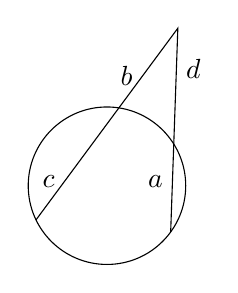
\begin{tikzpicture}
    \draw (0,0) circle (1cm);
    \draw [thin](0.8090169943749475,-0.5877852522924731)--(0.9,2)node[left,pos=0.25]{$a$} node[right,pos=0.8]{$d$}--(-0.9009688679024191,-0.4338837391175581)node[left,pos=0.25]{$b$} node[left,pos=0.8]{$c$};
\end{tikzpicture}&

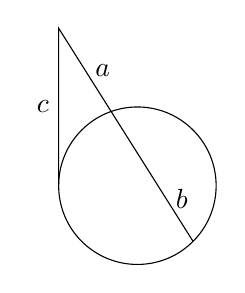
\begin{tikzpicture}
    \draw (0,0) circle (1cm);
    \draw [thin](-1,0)--(-1,2)node[left,pos=0.5]{$c$}--(0.7071067811865476,-0.7071067811865476)node[right,pos=0.2]{$a$} node[right,pos=0.8]{$b$};
\end{tikzpicture}\\
\hline
\end{tabular}
\label{table:CircleSegments}
\end{table}

\begin{enumerate}
    \item If two chords intersect, then the product of segments of one chord is equal to the product of segments of the other
    \item If 2 tangents are drawn to a circle from the same external point, then the tangents are equal
    \item If two secants are drawn to a circle from the same external point, then the product of the secant and its external segment equals the product of the other secant and its external segment
    \item If a tangent and secant are drawn to a circle from the same external point, then the tangent is the geometric mean between the external segment of the secant and the secant
\end{enumerate}

\section*{Cartesian Geometry}
\begin{enumerate}
    \item Midpoint Formula: The coordinate of the midpoint of two points is equal to the element wise arithmetic means of the coordinates of the initial two points.
    \item Slope Formula for lines: The slope of a line can be computed as the difference between the ordinates divided by the difference in the abscissae.
    \item The Euclidean distance between two points in two dimensions is the positive root of the sum of squares for the abscissae and the ordinates.
    \item If the product of the slopes of two lines is equal to -1 then the two lines are perpendicular
    \item If the slope of a line is the negative reciprocal of the slope of another line, then the two lines are perpendicular.
    \item If the slope of two lines are equal, then the lines are parallel
\end{enumerate}
